\chapter{Partially Ordered Sets}\label{ch:posets}

Alice was surfing the web and found a site listing top movies, grouped
by categories (comedy, drama, family, etc) as well as by the decade in 
which they were released.  The top seven dramas,
at least according to the movie critic hosting the web site, were:

\begin{enumerate}
\item Saving Private Ryan 
\item Life is Beautiful 
\item Forrest Gump
\item Braveheart
\item Good Will Hunting
\item Titanic
\item Jurassic Park
\end{enumerate}

Alice was intrigued by the listing and decided to make her own.
For comparison purposes, she agreed to use the same set of films
but she felt that the following list was a more accurate ranking:

\begin{enumerate}
\item Life is Beautiful 
\item Saving Private Ryan 
\item Good Will Hunting
\item Titanic
\item Braveheart
\item Forrest Gump
\item Jurassic Park
\end{enumerate}

Bob listened carefully to Alice's rationale for her ranking, all the
while scratching on his notepad.  Eventually, he held up the following
diagram and offered it as a statement of those comparisons on which both Alice
and the movie critic were in agreement. 

\begin{figure}
\begin{center}
\includegraphics*[scale=.4]{posets-figs/newfig-1.pdf}
\caption{Top Movies from the 90's}
\label{fig:movies}
\end{center}
\end{figure}

Do you see how Bob made up this diagram?  Add your own rankings of these
seven films and then draw the diagram that Bob would produce as a statement
about the comparisons on which you, Alice and the movie critic were in agreement.

More generally, when humans are asked to express preferences among 
a set of options, they often report that establishing a totally ranked list 
is difficult if not impossible.  Instead, they prefer to report a partial 
order---where comparisons are made between certain pairs of options but not 
between others.  In this chapter, we
make these observations more concrete by introducing the concept of 
a partially ordered set.  Examples include (1)~families of sets which are
partially ordered by inclusion, and (2)~a set of positive integers which is
partially ordered by division.  In computer science, file systems are 
modeled by trees which become partially ordered sets whenever links are added.

This chapter begins with a rapid survey of definitions and basic facts
not explicitly marked as propositions, lemmas, or theorems. In fact,
one could call them corollaries of the definitions. The validity of
most of these facts is immediately clear, but readers are strongly
encouraged to read \emph{actively} to understand \emph{why} each of
these statements is true.

\section{Basic Notation and Terminology}\label{s:posets:intro}

A \textit{partially ordered set} or \textit{poset} is a pair $(X,P)$
where $X$ is a set and $P$ is a reflexive, antisymmetric, and
transitive binary relation on $X$. (Refer to the appendix for a
refresher of what these properties are if you need to.) We call $X$
the \textit{ground set} while $P$ is a \textit{partial order} on
$X$. Elements of the ground set $X$ are also called \textit{points},
and the poset is \textit{finite} if the ground set is finite.  In our
class, we will be concerned almost exclusively with \textit{finite}
posets. To emphasize the order concept, we write $x\le y$ in $P$ and
$y\ge x$ in $P$ when $(x,y)\in P$. Of course, the notations $x<y$ in
$P$ and $y>x$ in $P$ mean $x\le y$ in $P$ and $x\ne y$. When the poset
remains fixed throughout a discussion, we will sometimes abbreviate
$x\le y$ in $P$ by just writing $x\le y$, etc.  If $x,y\in X$ and either $x<y$ or $y<x$, we
say $x$ and $y$ are \textit{comparable} in $P$; else
we say $x$ and $y$ are \textit{incomparable} in $P$.

A partial order $P$ is called a \textit{total} order (also, a 
\textit{linear} order) if for all $x,y\in X$, either $x\le y$ in $P$
or $y\le x$ in $P$.  For small finite sets, we can specify a linear
order by listing the elements from least to greatest.  For example,
$L=[b,c,d,a,f,g,e]$ is a linear order on the ground set $\{a,b,c,d,e,f,g\}$.
Note that $d <f$, $c<g$ and $e>b$ in $L$.  Also, note that the set of
real numbers comes equipped with a total order.  For example,
$1<7/5<\sqrt{2}<\pi$ in the natural total order on real numbers.  
But in this chapter, we will be interested
primarily with partial orders that are \textit{not} linear orders.

Let $\PXP$ be a poset and let $x$ and $y$ be distinct points from $X$.
We say $x$ is \textit{covered} by $y$ in $P$\footnote{Reflecting
the vagaries of the English language, many mathematicians use the
phrases: (1) $x$ is covered by $y$ in $P$; (2)~$y$ covers $x$ in
$P$; and (3)~$(x,y)$ is a cover in $P$ interchangeably.}
when $x<y$ in $P$, and there is no point $z\in X$ for
which $x<z$ in $P$ and $z<y$ in $P$.  Given a poset $\PXP$,
We can then define a \textit{cover graph} $\mathbf{G}$ whose vertex set
is $X$ with $xy$ an edge in $\mathbf{G}$ if and only if one of $x$
and $y$ covers the other in $\bfP$.

It is convenient to illustrate a
poset with a suitably drawn diagram of the cover
graph in the Euclidean plane.  We choose a standard
horizontal/vertical coordinate system in the plane and require that
the vertical coordinate of the point corresponding to $y$ be larger
than the vertical coordinate of the point corresponding to $x$
whenever $y$ covers $x$ in $P$. Each edge in the cover graph is represented
by a straight line segment which contains no point corresponding to any
element in the poset other than those associated with its two end points.
Such diagrams are called \textit{Hasse diagrams}
(\textit{poset diagrams, order diagrams}, or just \textit{diagrams}).

In \autoref{fig:poset-17pts},
we illustrate a poset with ground set $X=[17]=\{1,2,\dots,17\}$. 

\begin{figure}
\begin{center}
\includegraphics*[scale=.4]{posets-figs/wttfig-1}
\caption{A Poset on 17 Points}
\label{fig:poset-17pts}
\end{center}
\end{figure}

There are several quite natural ways to construct posets.  Here
are four such examples.
\begin{enumerate}
\item A family $\mathcal{F}$ of sets is partially ordered by
inclusion, i.e., set $A\le B$ if and only if $A$ is a subset of
$B$.
\item A set $X$ of positive integers is partially ordered by
division---without remainder, i.e., set $m\le n$ if and only if
$n\equiv 0\pmod{m}$.  
\item A set $X$ of $t$-tuples of real numbers is
partially ordered by the rule: \\
$(a_1,a_2,\dots,a_t)\le (b_1,b_2,\dots,b_t)$ if
and only if $a_i\le b_i$ in $\reals$ for $i=1,2,\dots,t$.  
\item When $L_1$, $L_2,\dots,L_k$ are linear orders on the same set
$X$, we can define a partial order $P$ on  $X$ by setting
$x\le y$ in $P$ if and only if $x\le y$ in $L_i$ for all $i=1,2,\dots,k$.
As is now clear, in the discussion at the very beginning of 
this chapter, Bob was drawing diagrams for the posets determined by 
the intersection of the linear orders given by Alice and the movie critic.
\end{enumerate}

% Let $\PXP$ be a poset.  
% 
% With a poset $\PXP$, we associate a \textit{comparability} graph
% ${\bfG}_1=(X,E_1)$, an \textit{incomparability} graph
% ${\bfG}_2=(X,E_2)$, and a \textit{cover }graph ${\bfG}_3=(X,E_3)$. The
% edges in the comparability graph ${\bfG}_1$ consist of the comparable
% pairs and the edges in the incomparability graph are the incomparable
% pairs. The edges of the cover graph consist of those pairs $xy$ for
% which $x<:y$ in $P$ or $y<:x$ in $P$.  Not every graph is a
% comparability graph.
% 
% In \autoref{fig:diagram}, we show a poset $\bfP$ and its associated
% comparability and incomparability graphs.
% 
% \begin{figure}
% \begin{center}
% \includegraphics*[scale=.4]{posets-figs/wttfig-6}
% \caption{Poset with Comparability and Incomparability Graphs}
% \label{fig:diagram}
% \end{center}
% \end{figure}

In fact, every finite poset arises from each of these four models.
We illustrate this with the poset shown in Figures~\ref{fig:inclusion},
\ref{fig:division} and~\ref{fig:prod-euclid} for the first three
examples, and leave the last an exercise.

\begin{figure}
\begin{center}
\includegraphics*[scale=.4]{posets-figs/wttfig-2}
\caption{An Inclusion Order}
\label{fig:inclusion}
\end{center}
\end{figure}

\begin{figure}
\begin{center}
\includegraphics*[scale=.4]{posets-figs/wttfig-3}
\caption{Positive Integers Ordered by Division}
\label{fig:division}
\end{center}
\end{figure}

\begin{figure}
\begin{center}
\includegraphics*[scale=.4]{posets-figs/wttfig-4}
\caption{The Product Order on Euclidean Space}
\label{fig:prod-euclid}
\end{center}
\end{figure}

When $\PXP$ is a poset and $Y\subseteq X$, the binary relation
$Q=P\cap(Y\times Y)$ is a partial order on $Y$, and we call the
poset $(Y,Q)$ a \textit{subposet} of $\bfP$.  Here are two
important classes of subposets.

When $\PXP$ is a poset and $C$ is a subset of $X$,
we say that $C$ is a \textit{chain} if every distinct pair of points 
from $C$ is comparable in $P$.  When $P$ is a linear order, the entire ground 
set $X$ is a chain.  Dually, if $A$ is a subset of $X$, we say that
$A$ is an \textit{antichain} if every distinct pair of points from $A$ 
is incomparable in $P$.  Note that a one-element subset
is both a chain and an antichain.  Also, we consider the emptyset as
both a chain and an antichain.

The \textit{height} of a poset
$(X,P)$, denoted $\height(P)$, is the largest $h$ for which there exists
a chain of $h$ points in $P$.
Dually, the \textit{width} of a poset $\PXP$, denoted $\width(P)$, is the
largest $w$ for which there exists an antichain of $w$ points in
$P$. 

\begin{question}
Given a poset $\PXP$, how hard is to determine its height and width?
\end{question}

Bob says that it is very easy.  For example, to find the width, just 
list all the subsets of $X$.  Delete those which are not antichains.
The answer is the size of the largest subset that remains.

Alice groans at Bob's naivety and suggests that he should read
further in this chapter.

\section{Additional Concepts for Posets}

We say $(X,P)$ and $(Y,Q)$ are \textit{isomorphic}, and write $(X,P)
\cong(Y,Q)$ if there exists a bijection (1--1 and
onto map) $f:X\to Y$ so that $x_1\le x_2$ in $P$ if and only if
$f(x_1)\le f(x_2)$ in $Q$. In this definition, the map $f$ is called an
\textit{isomorphism} from $\bfP$ to $\bfQ$. An isomorphism from $\bfP$ to 
$\bfP$ is called an \textit{automorphism} of $\bfP$. An isomorphism from 
$\bfP$ to a subposet of $\bfQ$ is called an \textit{embedding} of
$\bfP$ in $\bfQ$. In most settings, we will not distinguish between
isomorphic posets, and we will say that a poset $\PXP$ is \textit{contained}
in $\QYQ$ (also $\bfQ$ \textit{contains} $\bfP$) when there is an
embedding of $\bfP$ in $\bfQ$. Also, we will frequently say $\bfP=\bfQ$
when $\bfP$ and $\bfQ$ are isomorphic.

With the notion of isomorphism, we are lead naturally to the notion of
an ``unlabelled'' posets, and in \autoref{f:unlabelled}, we show a
diagram for such a poset.

\begin{figure}[hb]
\begin{center}
\includegraphics*[scale=.4]{posets-figs/wttfig-5.pdf}
\caption{\label{f:unlabelled}\sc An Unlabelled Partially Ordered Set}
\end{center}
\end{figure}

Note that the poset shown in \autoref{f:unlabelled} has the property
that there is only one maximal point.  Such a point is sometimes
called a \textit{one}, denoted not surprisingly as~$1$.  Also, there
is only one minimal point, and it is called a \textit{zero},
denoted~$0$.

The \textit{dual} of a partial order $P$ on a set $X$ is denoted by
$P^d$ and is defined by $P^d=\{(y,x):(x,y)\in P\}$. The \textit{dual}
of the poset $\PXP$ is denoted by $\bfP^d$ and is defined by
$\bfP^d=(X,P^d)$. A poset $\bfP$ is \textit{self-dual} if
$\bfP=\bfP^d$.

A poset $\PXP$ is \textit{connected} if for every $x,y\in X$ with
$x\ne y$, there is a finite sequence $x=x_0,x_1,\dots,x_n=y$ of points
from $X$ so that $x_i$ is comparable to $x_{i+1}$ in $P$ for
$i=0,1,2,\dots,n-1$. A subposet $(Y,P(Y))$ of $(X,P)$ is called a
\textit{component} of $\bfP$ if $(Y,P(Y))$ is connected and there is
no subset $Z\subseteq X$ containing $Y$ as a proper subset for which
$(Z,P(Z))$ is connected.  A one-point component is \textit{trivial}
(also, a \textit{loose} point or \textit{isolated} point); components
of two or more points are \textit{nontrivial}.  Note that a loose
point is both a minimal element and a maximal element.  Returning to
the poset shown in \autoref{fig:poset-17pts}, we see that it has two
components.

With a poset $\PXP$, we associate a \textit{comparability} graph
${\bfG}_1=(X,E_1)$, an \textit{incomparability} graph
${\bfG}_2=(X,E_2)$, and a \textit{cover }graph ${\bfG}_3=(X,E_3)$. The
edges in the comparability graph ${\bfG}_1$ consist of the comparable
pairs and the edges in the incomparability graph are the incomparable
pairs. The edges of the cover graph consist of those pairs $xy$ for
which $x<:y$ in $P$ or $y<:x$ in $P$.  Not every graph is a
comparability graph.  Also, not every graph is a cover graph.
Diagrams of posets are drawings of cover graphs---with additional
restrictions placed on the relative height of $x$ and $y$ when
$y$ covers $x$ in the poset.  On the other hand, there are no such
restrictions when drawing comparability and incomparability graphs.

In \autoref{fig:diagram}, we show a poset $\bfP$ and its associated
comparability and incomparability graphs.

\begin{figure}
\begin{center}
\includegraphics*[scale=.4]{posets-figs/wttfig-6}
\caption{Poset with Comparability and Incomparability Graphs}
\label{fig:diagram}
\end{center}
\end{figure}

\section{Dilworth's Chain Covering Theorem and its Dual}\label{s:posets:dilworth}

In this section, we prove the following theorem of R. P. Dilworth,
which is truly one of the classic results of combinatorial mathematics.

\begin{theorem}[Dilworth's Theorem]\label{thm:dilworth}
If $\PXP$ is a poset and $\width(X,P)=w$, then there exists a 
partition $X=C_1\cup C_2\cup\dots \cup C_w$, where $C_i$ is a 
chain for $i=1,2,\dots,w$. Furthermore, there is no chain partition
into fewer chains.
\end{theorem}

Before proceeding with the proof of Dilworth's theorem, we pause to
discuss the dual version for partitions into antichains, as it is
even easier to prove.

\begin{theorem}\label{thm:dualdilworth}
If $\PXP$ is a poset and $\height(P)=h$,
then there exists a partition $X=A_1\cup A_2\cup\dots\cup A_h$, where
$A_i$ is an antichain for $i=1,2,\dots,h$. Furthermore, there is no
partition using fewer antichains.
\end{theorem}

\begin{proof}
For each $x\in X$, let $\height(x)$ be the largest integer $t$ for
which there exists a chain \[x_1<x_2<\dots < x_t\] with $x=x_t$.
Evidently, $\height(x)\le h$ for all $x\in X$.  Then for each
$i=1,2,\dots,h$, let $A_i=\{x\in X:\height(x)=i\}$.  It is easy to
see that each $A_i$ is an antichain, as if $x,y\in A_i$ are such
that $x<y$, then there is a chain $x_1<x_2<\cdots<x_i=x <
x_{i+i}=y$, so $\height(y)=i+1$. Since $\height(P)=h$, there is a
maximum chain $C=\{x_1,x_2,\dots,x_h\}$. If it were possible to
partition $\bfP$ into $t<h$ antichains, then by the pigeonhole
principle, one of the antichains would contain two points from $C$,
but this is not possible.
\end{proof}

When $\PXP$ is a poset, a point $x\in X$ with $\height(x)=1$ is 
called a \textit{minimal} point of $\bfP$.  We denote the set of all minimal
points of a poset $\PXP$ by $\min(X,P)$ \footnote{Since we use the
notation $\bfP= (X,P)$ for a poset, the set of minimal elements can
be denoted by $ \min(\bfP)$ or $\min(X,P)$. This convention will be
used for all set valued and integer valued functions of posets.}.

The argument given for the proof of \autoref{thm:dualdilworth} yields
an efficient algorithm, one that is defined recursively.  Set $\bfP_0=
\bfP$.  If $P_i$ has been defined and $P_i\neq \emptyset$, let
$A_i=\min(\bfP_i)$ and then let $\bfP_{i+1}$ denote the subposet remaining
when $A_i$ is removed from $\bfP_i$.

In \autoref{fig:height=5}, we illustrate the antichain partition
provided by this algorithm.  Note that the poset used here
is the same poset appearing previously in \autoref{fig:poset-17pts}.

\begin{figure}
\begin{center}
\includegraphics*[scale=.4]{posets-figs/wttfig-7}
\caption{A Poset of Height 5}
\label{fig:height=5}
\end{center}
\end{figure}

\begin{remark}
Alice claims that it is very easy to find the set of minimal elements of
a poset.  Do you agree?
\end{remark}

Dually, we can speak of the set $\max(\bfP)$ of \textit{maximal} points
of $\bfP$.  We can also partition $\bfP$ into $\height(\bfP)$ antichains
by recursively removing the set of maximal points.

We pause to remark that when $\PXP$ is a poset, the set of all chains of
$\bfP$ is itself partially ordered by inclusion.  So it is natural to
say that a chain $C$ is \textit{maximal} when there is no chain
$C'$ containing $C$ as a proper subset.  Also, a chain $C$ is \textit{maximum}
when there is no chain $C'$ with $|C|<|C'|$.  Of course, a maximum chain
is maximal, but maximal chains need not be maximum.

Maximal antichains and maximum antichains are defined analogously.

With this terminology, the thrust of \autoref{thm:dualdilworth} is
that it is easy to find the height $h$ of a poset as well as a maximum
chain $C$ consisting of $h$ points from $\bfP$.

\subsection{Proof of Dilworth's Theorem}

The argument for Dilworth's theorem is simplified by the 
following notation. When $\PXP$ is a poset and $x\in X$, we let $D(x)=\{y\in 
X:y<x \text{ in }P\}$; $D[x]=\{y\in X:y\le x\text{ in }P\}$; $U(x)=\{y\in X:y>x
\text{ in }P\}$; $U[x]=\{y\in X:y\ge x\}$; and $I(x)=\{y\in X-\{x\}:x\Vert y
\text{ in }P\}$. When $S\subseteq  X$, we let $D(S)=
\{y\in X:y<x$ in $P$, for some $x\in S\}$ and $D[S]=S\cup D(S)$. The
subsets $U(S)$ and $U[S]$ are defined dually.  Note that when 
$A$ is a maximal antichain in $\bfP$, the ground set $X$ is
partitioned into pairwise disjoint sets:\quad $X=A\cup D(A)\cup U(A)$.

We are now ready for the proof.  Let $\PXP$ be a poset and let $w$ denote
the width of $\bfP$.
As in \autoref{thm:dualdilworth}, the pigeonhole principle implies
that we require at least $w$ chains in any chain partition of
$\bfP$. To prove that $w$ suffice, we
proceed by induction on $|X|$, the result being trivial if
$|X|=1$. Assume validity for all posets with $|X|\le k$ and suppose
that $\PXP$ is a poset with $|X|=k+1$. Without loss of generality,
$w>1$; else the trivial partition $X=C_1$ satisfies the
conclusion of the theorem. Furthermore, we observe that if $C$ is a
(nonempty) chain in $(X,P)$, then we may assume that the subposet
$(X-C,P(X-C))$ also has width $w$. To see this, observe that the
theorem holds for the subposet, so that if
$\width(X-C,P(X-C))=w'<w$, then we can partition $X-C$ as
$X-C=C_1\cup C_2\cup\dots\cup C_{w'}$, so that $X=C\cup
C_1\cup\dots\cup C_{w'}$ is a partition into $w'+1$ chains. Since
$w'<w$, we know $w'+1\le w$, so we have a partition of $X$ into at
most $w$ chains. Since any partition of $X$ into chains must use at
least $w$ chains, this is exactly the partition we seek.

Choose a maximal point $x$ and a minimal point $y$ with $y\le x$ in
$P$. Then let $C$ be the chain containing $x$ and $y$. Note that
$C$ contains either one or two elements depending on whether $x$
and $y$ are distinct.

Let $Y=X-C$ and  $Q=P(Y)$ and let $A$ be a $w$ element antichain
in the  subposet $(Y,Q)$.  In the partition $X=A\cup D(A)\cup U(A)$, the
fact that $y$ is a minimal point while $A$ is a maximal
antichain imply that $y\in D(A)$.  Similarly, $x\in U(A)$.  In particular,
this shows that $x$ and $y$ are distinct.

Label the elements of $A$ as
$\{a_1,a_2,\dots,a_w\}$. Note
that $U[A]\ne X$ since $y\notin U[A]$, and $D[A]\ne X$ since
$x\notin D[A]$. Therefore, we may apply the inductive hypothesis to
the suposets of $\bfP$ determined by $D[A]$ and $U[A]$, respectively,
and partition each of these two subposets into $w$ chains: 

\[
U[A]= C_1\cup C_2\cup\dots\cup C_w\quad\text{and}\quad
 D[A]=D_1\cup D_2\cup\dots\cup D_w
\]
Without loss of generality, we may assume these chains have
been labeled so that $a_i\in C_i\cap D_i$ for each $i=1,2,\dots,w$. 
However, this implies that 
\[
X=(C_1\cup D_1)\cup (C_2\cup D_2)\cup\dots\cup(C_w\cup D_w)
\]
is the desired partition which in turn completes the proof.

In \autoref{fig:width=7}, we illustrate Dilworth's chain covering
theorem with a poset of width~$7$ that has been partitioned into~$7$
chains.

\begin{figure}
\begin{center}
\includegraphics*[scale=.4]{posets-figs/wttfig-8}
\caption{A Poset of Width 7}
\label{fig:width=7}
\end{center}
\end{figure}

\begin{remark}
The ever alert Alice notes that
the proof given above for Dilworth's theorem does not seem to provide
an efficient algorithm for finding the width~$w$ of a poset, much less
a partition of the poset into $w$ chains.  Bob has yet to figure out
why listing all the subsets of $X$ is a bad idea.  We will return to 
this issue later in the course.
\end{remark}

\section{Linear Extensions of Partially Ordered Sets}\label{s:posets:sorting}

Let $\PXP$ be a partially ordered set.  A linear order $L$ on $X$ is
called a \textit{linear extension} (also, a \textit{topological sort})
of $P$, if $x<y$ in $L$ whenever $x<y$ in $P$.  For example, the
poset shown in \autoref{fig:posets:lin-extn} and has~11 linear extensions.

\begin{figure}[h]
\begin{center}
\begin{minipage}{.25\textwidth}
\begin{overpic}[scale=.4]{posets-figs/wttfig-9}
\put(-3,2){$z$}
\put(48,32.5){$w$}
\put(48,2){$a$}
\put(-3,32.5){$b$}
\put(48,63){$c$}
\put(48,93){$d$}
\end{overpic}\hspace{.5in}
\end{minipage}
\begin{minipage}{.70\textwidth}
\[
\begin{array}{ccccccccccc}
L_1& L_2 & L_3 & L_4 & L_5 & L_6 & L_7 & L_8 & L_9 & L_{10} & L_{11}\\[.2in]
% \vspace{.2in}
 d & d & d & b & d & d & d & b & d & d & b \\
 c & c & b & d & c & c & b & d & c & b & d \\
 w & b & c & c & w & b & c & c & b & c & c \\
 b & w & w & w & b & w & w & w & z & z & z \\
 a & a & a & a & z & z & z & z & w & w & w \\
 z & z & z & z & a & a & a & a & a & a & a \\
\end{array}
\]
\end{minipage}
\caption{\label{fig:posets:lin-extn}A poset and its linear extensions}
\end{center}
\end{figure}

The classical sorting problem studied in all elementary computer
science courses is to determine an unknown linear order $L$ of a set $X$
by asking a series of questions of the form:\quad Is $x<y$ in $L$?

Here is an important special case: determine an unknown linear 
extension $L$ of a poset $\bfP$ by asking a series of questions of the form:
\quad Is $x < y$ in $L$? 

\begin{question}
Given a poset $\PXP$ and the problem of determining an unknown linear
extension of $P$, how should you decide which question (of the
form:\quad Is $x<y$ in $L$?) to ask?
\end{question}

\section{The Subset Lattice}\label{s:posets:subset-lattice}

When $X$ is a finite set, the family of all
subsets of $X$ forms a \textit{subset lattice}.  We illustrate this
in \autoref{fig:subset-lattice} where we show the lattice
of all subsets of $\{1,2,3,4\}$. In this figure, note that we
are representing sets by bit strings, and we have further abbreviated
the notation by writing strings without commas and parentheses.

\begin{figure}
\begin{center}
\includegraphics*[scale=.4]{posets-figs/wttfig-10}
\caption{A Subset Lattice}
\label{fig:subset-lattice}
\end{center}
\end{figure}

For a positive integer $t$, we let $\bftwo^t$ denote the subset
lattice consisting of all subsets of $\{1,2,\dots,t\}$
ordered by inclusion.  Some elementary properties of this
poset are:

\begin{enumerate}
\item The height is $t+1$ and all maximal chains have exactly
$t+1$ points.
\item The size of the poset $\bftwo^t$ is $2^t$ and the elements
are partitioned into ranks (antichains) $A_0, A_1,\dots, A_t$
with $|A_i|=\binom{t}{i}$ for each $i=0,1,\dots,t$.
\item The maximum size of a rank in the subset lattice occurs
in the middle, i.e. if $s=\lfloor t/2\rfloor$, then the
largest binomial coefficient in the sequence $\binom{t}{0},
\binom{t}{1},\binom{t}{2},\dots,\binom{t}{t}$ is $\binom{t}{s}$.
Note that when $t$ is odd, there are two ranks of maximum size,
but when $t$ is even, there is only one.
\end{enumerate}

\subsection{Sperner's Theorem}\label{ss:posets:subset-lattice:sperner}

For the width of the subset lattice, we have the following
classic result due to Sperner.

\begin{theorem}[Sperner]\label{thm:sperner}
For each $t\ge1$, the width of the subset lattice $\bftwo^t$
is the maximum size of a rank, i.e., 
\[
\width(\bf2^t)=\binom{t}{\lfloor\frac{t}{2}\rfloor}
\]
\end{theorem}

\begin{proof}
The width of the poset $\bftwo^t$ is at least
$C(t,\lfloor\frac{t}{2}\rfloor)$ since the set of all
$\lfloor\frac{t}{2}\rfloor$-element subsets of $\{1,2,\dots,t\}$ is an
antichain.  We now show that the width of $\bftwo^t$ is at most
$C(t,\lfloor\frac{t}{2}\rfloor)$.

Let $w$ be the width of $\bftwo^t$ and let $\{S_1,S_2,\dots, S_w\}$ be
an antichain of size $w$ in this poset, i.e., each $S_i$ is a subset
of $\{1,2,\dots,t\}$ and if $1\le i<j\le w$, then $S_i\nsubseteq
S_j$ and $S_j\nsubseteq S_i$.

For each $i$, consider the set $\cgS_i$ of all maximal chains which
pass through $S_i$.  It is easy to see that if $|S_i|=k_i$, then
$|\cgS_i|=k_i!(t-k_i)!$.  This follows from the observation that to
form such a maximum chain beginning with $S_i$ as an intermediate
point, you delete the elements of $S_i$ one at a time to form the
sets of the lower part of the chain.  Also, to form the upper part
of the chain, you add the elements not in $S_i$ one at a time.

Note further that if $1\le i <j\le w$, then $\cgS_i\cap \cgS_j
=\emptyset$, for if there was a maximum chain belonging to both
$\cgS_i$ and $\cgS_j$, then it would imply that one of $S_i$ and
$S_j$ is a subset of the other.

Altogether, there are exactly $t!$ maximum chains in $\bftwo^t$.  This
implies that
\[\sum_{i=1}^{i=w} k_i!(t-k_i)!\le t!.\]
This implies that
\[\sum_{i=1}^{i=w}\frac{k_i!(t-k_i)!}{t!}=
\sum_{i=1}^{i=w}\frac{1}{\binom{t}{k_i}}\le 1. 
\]
It follows that
\[
\sum_{i=1}^{i=w}\frac{1}{\binom{t}{\lceil\frac{t}{2}\rceil}}\le 1
\]
Thus
\[
w\le \binom{t}{\lceil\frac{t}{2}\rceil}.
\]
\end{proof}

\section{An Alternative Proof of Sperner's Theorem}

A poset $\PXP$ is said to be \textit{ranked} if all maximal
chains have the same cardinality.  When a poset is ranked,
then there is a partition $X=A_1\cup A_2\cup \dots A_h$
so that every maximal chain consists of exactly one point from
each $A_i$. We call this partition its \textit{partition into ranks}.

A ranked poset is said to be \textit{sperner} if the width of the
poset is just the maximum cardinality of a rank.  The preceding
theorem can now be reinterpreted as saying that the subset lattice is
a sperner poset.  Let $(X,P)$ be a ranked poset of height $h$ and let
$X= A_1\cup A_2\cup \dots A_h$ be its partition into ranks.  A chain
$C=\{x_1,x_2,\dots,x_k\}$ in $(X,P)$ is called a \textit{symmetric}
chain if there exists an integer $s$ so that $C$ contains exactly one
point from each rank $A_s,A_{s+1},\dots,A_{h+1-s}$.  Intuitively, a
symmetric chain is balanced about the middle of the poset $(X,P)$ and
dense in the sense that it is not possible to insert a point in
between two consecutive points in $C$.

The following proposition is self evident.

\begin{proposition}\label{prop:symmchain-sperner}
If a ranked poset has a partition into symmetric chains,
then it is a sperner poset.  In fact, its width is
just the size of the middle rank(s).
\end{proposition}

Here is an alternative proof of Sperner's theorem.

\begin{theorem}\label{thm:subset-lattice-symmchain}
For each $t\ge1$, the subset lattice $\bftwo^t$ has a symmetric chain
partition.
\end{theorem}

We actually prove an even stronger result.  For posets $\PXP$ and
$\QYQ$, we define the \textit{cartesian product} $\bfP\times \bfQ$ as
follows.  The point set $X\times Y$ with $(x_1,y_1)\le (x_2,y_2)$ in
$\bfP\times \bfQ$ if and only if $x_1\le x_2$ in $\bfP$ and $y_1\le
y_2$ in $\bfQ$.  Note that the subset lattice $\bftwo^t$ is just the
cartesian product $\bftwo\times\bftwo\times\dots\times\bftwo$, with a total
of $t$ factors of $\bftwo$.

\begin{lemma}\label{lem:prodchain-symmchain}
Let $m$ and $n$ be positive integers.  Then
the cartesian product $\bfm\times\bfn$ has
a symmetric chain partition.
\end{lemma}

\begin{proof}
The point set of $\bfm\times\bfn$ is just
$\{(i,j):0\le i <m, 0\le j<n\}$.  
Without loss of generality $m\le n$, so that
the width of $\bfm\times\bfn$ is $m$.  Then
for each $i=0,1,\dots,m-1$, let 
\[
C_i=\{(i,0),(i,1),\dots,(i,n-1-i),(i+1,n-1-i),\dots,(m-1,n-1-i)\}.
\]
Then the family $\{C_1,C_2,\dots,C_m\}$ is
a symmetric chain partition of $\bfm\times\bfn$.
\end{proof}

\begin{theorem}\label{thm:ranked-prod-symmchain}
If $\bfP$ and $\bfQ$ are ranked posets and each has
a symmetric chain partition, then $\bfP\times\bfQ$
is ranked and has a symmetric chain partition.
\end{theorem}

\begin{proof}
It is easy to see that if $\bfP$ is ranked and has
height $h_1$ and $\bfQ$ is ranked and has height $h_2$,
then $\bfP\times\bfQ$ is ranked and has height
$h_1+h_2-1$.  Now suppose that $\bfP$ and $\bfQ$ have
symmetric chain partitions.  Let $C$ be a chain from
the partition of $\bfP$ and let $D$ be a chain from
the partition of $\bfQ$.  Then apply the preceding lemma
to obtain a partition of the product $C\times D$.
What results is a saturated partition of $\bfP\times
\bfQ$.
\end{proof}

\section{Dedekind's Problem}\label{s:posets:subset-lattice:dedekind}

The problem of counting the number $A(t)$ of antichains 
in the subset lattice $\bftwo^t$ is a famous problem known 
in the literature as Dedekind's problem.  Here is a table of 
the numbers which have been computed.
\begin{align*}
A(1)&=3\\
A(2)&=6\\
A(3)&=20\\
A(4)&=168\\
A(5)&=7781\\
A(6)&=7828354\\
A(7)&=2414682040998\\
A(8)&=56130437228687557907788
\end{align*}
Perhaps, the calculation of $A(10)$ is beyond reach.

\section{Interval Orders}\label{s:posets:intervalorder}

When we discussed Dilworth's theorem, we commented that the
algorithmic aspects would be deferred until later in the text.  But
there is one important class of orders for which the full solution is
easy to obtain.

A poset $\PXP$ is called an \textit{interval order} if there
exists a function $I$ assigning to each element $x\in X$ a closed
interval $I(x)=[a_x,b_x]$ of the real line $\reals$ so that for
all $x$, $y\in X$, $x<y$ in $P$ if and only if $b_x<a_y$ in $L$.
We call $I$ an \textit{interval representation}
of $\bfP$, or just a \textit{representation} for short.
For brevity, whenever we say that $I$ is a representation of an
interval order $\PXP$, we will use the alternate notation $[a_x,b_x]$ for
the closed interval $I(x)$.  Also, we let $|I(x)|$ denote the
\textit{length} of the interval, i.e., $|I(x)|=b_x-a_x$. 
The poset shown first in \autoref{fig:diagram} above is
an interval order as the representation given in
\autoref{fig:intervalorder} verifies.

\begin{figure}
\begin{center}
\includegraphics*[scale=.4]{posets-figs/wttfig-11}
\caption{An interval order and its representation}
\label{fig:intervalorder} 
\end{center}
\end{figure}

Note that end points of intervals used in a representation
need not be distinct.  In fact, distinct points $x$ and $y$ from
$X$ may satisfy $I(x)=I(y)$.  We even allow degenerate intervals.
On the other hand, a representation is said to be
\textit{distinguishing} if all intervals are non-degenerate and
all end points are distinct. It is easy to see that every interval
order has a distinguishing representation. In fact, since we are
concerned only with finite posets, we could have just as well
required that all intervals used in the representation be open.

\begin{theorem}[Fishburn]\label{thm:fishburn}
Let $\PXP$ be a poset.  Then $\bfP$ is an interval order if 
and only if it does not contain $\bftwo+\bftwo$ as a subposet.
\end{theorem}

\begin{proof}
Suppose first that $\{x,y,z,w\}\subseteq X$ and the subposet
determined by these four points is isomorphic to $\bftwo+\bftwo$.
We show that $\bfP$ is not an interval order.  Suppose to the
contrary that $\bfP$ is an interval order and let $I$ be
an interval representation of $\bfP$.  Without loss of generality, we
may assume that $x<y$ and $z<w$ in $P$.  Thus $x\Vert w$ and
$z\Vert y$ in $P$.  Then $b_x<a_y$ and $b_z < a_w$ in $\reals$ 
so that $a_w \le b_x <a_y \le b_z$, which is a contradiction.

Next, we assume that $\bfP$ does not contain $\bftwo+\bftwo$ as a
subposet and show that $\bfP$ is an interval order.  We proceed by
induction on $n=|X|$.  The result is trivially true when $n=1$.  Now
assume that the result holds for all $n$ with $n\le k$, where $k$ is
some positive integer, and suppose that $|X|=k+1$.  Then among the
maximal elements, choose one which is greater than as many other
elements of $\bfP$ as possible.  Denote this element by $x_0$, and let
$\bfQ$ denote the subposet obtained by removing $x_0$ from $\bfP$.
Then $\bfQ$ has $k$ points and does not contain a subposet isomorphic
to $\bftwo+\bftwo$.  Therefore $\bfQ$ is an interval order.  Let $I$
be an interval representation of $\bfQ$.

Choose a real number $r$ with $r > b_y$ for every $y\neq x_0$.  If
$x_0$ is comparable to all other elements of $X$, then we may extend
$I$ to all of $X$ by simply taking $I(x_0) = [r,r+1]$.  Hence, we may
assume that the set $S=\{y\in X:x_0\Vert y$ in $P\}$ is non-empty.

\begin{claim*}
We have $S\subseteq \max(P)$.
\end{claim*}

\textit{Proof.}  Since $x_0$ is maximal and $x_0\|y$ for all $y\in S$,
it is enough to prove that $S$ is an antichain. Suppose to the
contrary that $y_1,y_2\in S$ and $y_1<y_2$.  Choose a maximal element
$y_3\in X$ with $y_2\le y_3$ in $P$.  Evidently, $y_3\neq x_0$, as
$x_0\| y_2$ but $y_2\leq y_3$.  Since $x_0$ is greater than as many
elements of $\bfP$ as possible, there must be some $u\in X$ with $u<x_0$
in $P$ and $u\| y_3$.  Now we have that $x_0\geq u$, $y_3\geq y_1$,
$x_0\|y_1$, $x_0\| y_3$, and $y_3\| u$ immediately from our choices of
these points. Furthermore, in order to preserve $x_0\| y_1$ and
$u\|y_3$, we cannot have $u\perp y_1$. Therefore, it follows that
$\{u,x_0,y_1,y_3\}$ determine a subposet isomorphic to
$\bftwo+\bftwo$.  This completes the proof of the claim.

\medskip
Now we modify the interval representation as follows:

\begin{equation*}
\widehat{I}(u)=
\begin{cases}
I(u)&\text{if $u\notin S$ and $u\neq x_0$};\\
[a_u,r]&\text{if $u\in S$};\\ 
[r,r+1]&\text{if $u = x$}.
\end{cases}
\end{equation*}

It is easy to see that $\widehat{I}$ is an interval representation of
$\bfP$.
\end{proof}

\section{Finding a Representation of an Interval Order}
\label{s:posets:intervalorder:findrep}

When $\PXP$ is an interval order and $n$ is a positive integer, there
may be many different ways to represent $\bfP$ using intervals with
integer end points in $[n]$.  But there is certainly a least $n$ for
which a representation can be found, and here the representation is
unique.  The discussion will again make use of the notation for down
sets and up sets that we introduced prior to the proof of Dilworth's
Theorem. As a reminder, we repeat it here. For a poset $\PXP$ and a
subset $S\subset X$, let $D(S) = \{y\in X:$ there exists some $x\in S$
with $y<x$ in $P\}$.  Also, let $D[S]=D(S)\cup S$.  When $|S|=1$, say
$S=\{x\}$, we write $D(x)$ and $D[x]$ rather than $D(\{x\})$ and
$D[\{x\}]$.  Dually, for a subset $S\subseteq X$, we define $U(S) =
\{y\in X:$ there exists some $x\in X$ with $y>x$ in $P\}$.  As before,
set $U[S]=U(S)\cup S$.  And when $S=\{x\}$, we just write $U(x)$ for
$\{y\in X:x<y$ in $P\}$.

Let $\PXP$ be a poset and let
\[
\mathcal{D} = \{D(x):x\in X\}\quad\text{ and }\quad
\mathcal{U} = \{U(x):x\in X\}
\]

Here are several elementary propositions which
follow easily from Fishburn's theorem.

\begin{proposition}\label{prop:char-intord}
Let $\PXP$ be a poset.  Then the following statements
are equivalent.
\begin{enumerate}
\item $\bfP$ is an interval order.
\item Any two distinct sets in $\mathcal{D}$ are ordered by inclusion.
\item Any two distinct sets in $\mathcal{U}$ are ordered by inclusion.
\end{enumerate}
\end{proposition}

\begin{proposition}\label{prop:intord-up=down}
When $\bfP$ is an interval order,
$|\mathcal{D}|=|\mathcal{U}|$.
\end{proposition}

Let $\bfP$ be an interval order and let $d=|\mathcal{D}|$.
Then label the sets in $\mathcal{D}$ and $\mathcal{U}$ respectively as
$D_1$, $D_2,\dots,D_d$ and $U_1$, $U_2,\dots,U_d$ 
so that
\[
\emptyset= D_1\subset D_2\subset D_3\subset\dots\subset D_d
 \quad\text{and}
\]
\[
U_1\supset U_{2}\cdots \supset U_{d-2}\supset U_{d-1}\supset\dots\supset U_d
 =\emptyset.
\]
Then we can form an interval representation $I$ of $\bfP$ by the
following rule:  For each $x\in X$, set $I(x)=[i,j]$, where
$D(x)=D_i$ and $U(x)=U_j$.

\begin{proposition}\label{prop:intord-minrep}
Let $\bfP$ be an interval order, and let $d=|\mathcal{D}|$
and $I$ be defined as above.  Then
\begin{enumerate}
\item For each $x\in X$, if $I(x)=[i,j]$, then $i\le j$ in $\mathbb{R}$.
\item For each $x,y\in X$, if $I(x)=[i,j]$ and $I(y)=[k,l]$, then
$x<y$ in $P$ if and only if $j<k$ in $\mathbb{R}$.
\item The integer $d$ is the least positive integer for which
$\bfP$ has an interval representation using integer end points
from $[d]$.  This representation is unique.
\end{enumerate}
\end{proposition}

Consider the poset shown in \autoref{fig:10intervalorder}.

\begin{figure}
\begin{center}
\includegraphics*[scale=.4]{posets-figs/wttfig-12}
\caption{An interval order on 10 Points}
\label{fig:10intervalorder} 
\end{center}
\end{figure}

Then $d= 5$ with 
$D_1=\emptyset$, $D_2=\{3\}$, $D_3=\{3,6,7\}$, $D_4=\{3,6,7,8\}$, and 
$D_5=\{1,3,6,7,8,10\}$.  Also
$U_1=\{1,2,4,5,8,9,10\}$, $U_2=\{1,2,5,8,9,10\}$,
$U_3=\{2,5,9\}$, $U_4=\{5\}$, and $U_5=\emptyset$.
So
\begin{align*}
I(1) &= [3,4]\\
I(2) &= [4,5]\\
I(3) &= [1,1]\\
I(4) &= [2,5]\\
I(5) &= [5,5]\\
I(6) &= [1,2]\\
I(7) &= [1,2]\\
I(8) &= [3,3]\\
I(9) &= [4,5]\\
I(10) &= [3,4]
\end{align*}

Also, this method yields an efficient algorithm for testing
whether a poset is an interval order.  You simply record the
down sets in $\mathcal{D}$ and see if they are ordered by
inclusion.  When a poset is not an interval order, you will
find distinct points $x$ and $y$ for which $D(x)\nsubseteq D(y)$
and $D(y)\nsubseteq D(x)$.  This implies that there exist
distinct points $z$ and $w$ with
$z\in D(x)-D(y)$ and $w\in D(y)-D(x)$.  The four points $x$, $y$,
$z$ and $w$ are then seen to form a copy of $\bftwo+\bftwo$. 

To illustrate this concept, erase the line joining points
$3$ and $10$ in the figure above.  You will then
find that $D(10)=\{6,7\}$ and $D(4)=\{3\}$.  Therefore
in $3$, $4$, $6$ and $10$ form a copy of $\bftwo+\bftwo$ in this
modified poset.

\section{Dilworth's Theorem for Interval Orders}\label{s:posets:dilworth-intord}

As remarked previously, we do not yet have an efficient
process for determining the width of a poset and a minimum
partition into chains.  For interval orders, there is indeed
a simple way to find both. The explanation is just to establish
a connection with coloring of interval graphs as discussed in
Chapter~$4$.

Let $\PXP$ be an interval order and let 
$\{[a_x,b_x]:x\in X\}$ be intervals of the real line
so that $x<y$ in $\bfP$ if and only $b_x<a_y$.
Then let $\bfG$ be the interval graph determined by this
family of intervals.  Note that if $x$ and $y$ are distinct
elements of $X$, then $x$ and $y$ are incomparable in $\bfP$ if and
only if $xy$ is an edge in $\bfG$.  In other words, $\bfG$ is
just the incomparability graph of $\bfP$.

Recall from Chapter~$4$ that interval graphs are perfect, i.e.,
$\chi(\bfG)=\omega(\bfG)$ for every interval graph $\bfG$.  Furthermore,
you can find an optimal coloring of an interval graph by applying first fit
to the vertices in a linear order that respects left end points.
Such a coloring concurrently determines a partition of $\bfP$ into
chains.

In fact, if you want to skip the part about interval representations,
take any linear ordering of the elements as $x_1$, $x_2,\dots,x_n$ so that
$i<j$ whenever $D(x)$ is a proper subset of $D(y)$.  Then apply First
Fit with respect to chains.  For example, using
the $10$ point interval order illustrated in \autoref{fig:10intervalorder},
here is such a labeling: 

\[\begin{array}{ccccc}
x_1 =7 &
x_2 =6 &
x_3 =3 &
x_4 =4 &
x_5 =8\\
x_6 =1 &
x_7 =10 &
x_8 =2 &
x_9 =9 &
x_{10} =5
\end{array}\]
Now apply the \textbf{First Fit} algorithm to the points of $\bfP$,
in this order, to assign them to chains $C_1$, $C_2,\dots$.  In other
words, assign $x_1$ to chain~$C_1$.  Thereafter if you have
assigned points $x_1$, $x_2,\dots,x_i$ to chains, then assign
$x_{i+1}$ to chain $C_j$ where $j$ is the least positive integer
for which $x_{i+1}$ is comparable to $x_k$ whenever $1\le k\le i$ and
$x_k$ has already been assigned to $C_j$.
For example, this rule results in the following chains for the
interval order $\bfP$ shown in \autoref{fig:10intervalorder}.

\begin{align*}
C_1 &= \{7,8,2\}\\ 
C_2 &= \{6,1,5\}\\
C_3 &= \{3,4\}\\
C_4 &= \{10\}\\
C_5 &= \{9\}
\end{align*}
In this case, it is easy to see that the chain partition is
optimal since the width of $\bfP$ is $5$ and $A=\{1,2,4,9,10\}$
is a $5$-element antichain.

But students should be very careful in applying First Fit to find optimal
chain partitions of posets---just as one must be leary of using First Fit
to find optimal colorings of graphs.  In general, there is always \textit{some}
linear ordering of the elements of the ground set for which First Fit will
work.  However, there is no known method for finding such a linear order,
and it might well be a hopelessly difficult assignment.

\section{Exercises}

\begin{enumerate}
\item We say that a relation $R$ on a set $X$ is \textit{symmetric} if
  $(x,y)\in R$ implies $(y,x)\in R$ for all $x,y\in X$. If
  $X=\{a,b,c,d,e,f\}$, how many symmetric relations are there on $X$?
  How many of these are reflexive?
\item A relation $R$ on a set $X$ is an \textit{equivalence relation}
  if $R$ is reflexive, symmetric, and transitive. Fix an integer
  $m\geq 2$. Show that the relation defined on the set
  $\ints$ of integers by $aRb$ ($a,b\in\ints$) if and only if $a\equiv
  b\pmod{m}$ is an equivalence relation. (Recall that $a\equiv
  b\pmod{m}$ means that when dividing $a$ by $m$ and $b$ by $m$ you
  get the same remainder.)
\item Is the binary relation \[P=\{(1,1),(2,2),(3,3),(4,4),(1,3),(2,4),(2,5),(4,5),(3,5),(1,5)\}\] a partial
  order on the set $X=\{1,2,3,4,5\}$? If so, discuss what properties
  you verified and how. If not, list the ordered pairs that must be
  added to $P$ to make it a partial order or say why it cannot be made
  a partial order by adding ordered pairs.
\item Draw the diagram of the poset $\bfP=(X,P)$ where
  $X=\{1,2,3,5,6,10,15,30\}$ and $x\leq y$ in $P$ if and only if
  $x|y$. (Recall that $x|y$ means that $x$ evenly divides $y$ without
  remainder. Equivalently $x|y$, if and only if $y\equiv
  0\pmod{x}$.) \label{exer:posets:division}
\item Draw the diagram of the poset $\PXP$ where
 \begin{multline*}
    X=\{\{1,3,4,5,6\},\{1,2,4,5,6\},\{1,2,3,6\},\{1,2,3\},\{1,5,6\},\\\{1,3,6\},\{1,2\},\{1,6\},\{3,5\},\{1\},\{3\},\{4\}\}
  \end{multline*}
 and $P$ is the partial order on $X$ given by the ``is a subset of''
 relationship.
\item A \textit{linear extension} of a poset $\bfP=(X,P)$ is a total
  order $L$ on $X$ such that if $x\leq y$ in $P$, then $x\leq y$ in $L$. Give a
  linear extension of the poset $\bfP$ in
  \hyperref[exer:posets:division]{Exercise~\ref*{exer:posets:division}}. How
  many linear extensions of $\bfP$ are there? (Do \textbf{not} just
  list them all.)
\item Alice and Bob are considering posets $\bfP$ and $\bfQ$. They
  soon realize that $\bfQ$ is isomorphic to $\bfP^d$. After $10$
  minutes of work, they figure out that $\bfP$ has height $5$ and
  width $3$. Bob doesn't want do find the height and width of $\bfQ$,
  since he figures it will take (at least) another $10$ minutes to
  answer these questions for $\bfQ$. Alice says Bob is crazy and that
  she already knows the height and width of $\bfQ$. Who's right and
  why?  
\item For this exercise, consider the poset $\bfP$ in \autoref{fig:poset-17pts}.
  \begin{enumerate}
  \item List the maximal elements of $\bfP$.
  \item List the minimal elements of $\bfP$.
  \item Find a maximal chain with two points in $\bfP$.
  \item Find a chain in $\bfP$ with three points that is \emph{not}
    maximal. Say why your chain is not maximal.
  \item Find a maximal antichain with four points in $\bfP$.
  \end{enumerate}
\item Find the height $h$ of the poset $\PXP$ shown below as well as a
  maximum chain and a partition of $X$ into $h$ antichains using the
  algorithm from this chapter.
  \begin{center}
    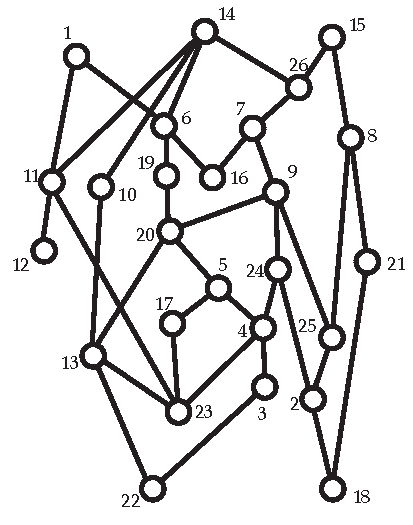
\includegraphics{posets-figs/height_ex_poset}
  \end{center}
\item Find the width $w$ of the poset in \autoref{fig:division}, an
  antichain of size $w$, and a partition of the ground set into $w$
  chains.
\item A restaurant chef has designed a new set of dishes for his
  menu. His set of dishes contains $10$ main courses, and he will
  select a subset of them to place on the menu each night. To ensure
  variety of main courses for his patrons, he wants to guarantee that
  a night's menu is neither completely contained in nor completely
  contains another night's menu. What is the largest number of menus
  he can plan using his $10$ main courses subject to this requirement?
\item Draw the diagram of the interval order represented in
  \autoref{fig:intord_to_diag_ex}.
  \begin{figure}[h]
  \begin{center}
    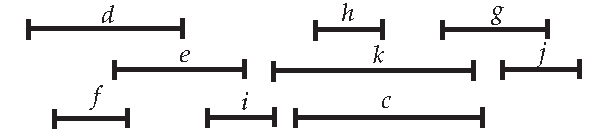
\includegraphics{posets-figs/intord_to_diag_ex}
  \end{center}
  \caption{An interval representation}\label{fig:intord_to_diag_ex}
  \end{figure}
\item Draw the diagram of the interval order represented in
  \autoref{fig:intord_to_diag_ex2}.
  \begin{figure}[h]
  \begin{center}
    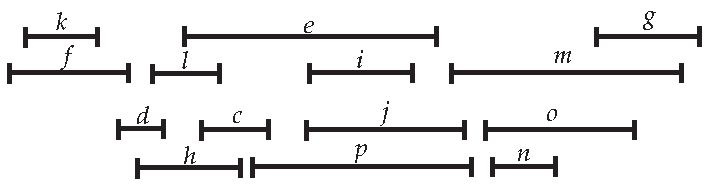
\includegraphics{posets-figs/intord_to_diag_ex2}
  \end{center}
  \caption{An interval representation}\label{fig:intord_to_diag_ex2}
  \end{figure}
\item Find an interval representation for the poset in
  \autoref{fig:intord_find_rep_ex1} or give a reason why one does not
  exist.
  \begin{figure}[h]
  \begin{center}
    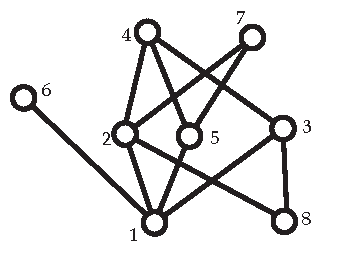
\includegraphics{posets-figs/intord_find_rep_ex1}
  \end{center}
  \caption{Is this poset an interval order?}\label{fig:intord_find_rep_ex1}
  \end{figure}
\item Find an interval representation for the poset in
  \autoref{fig:intord_find_rep_ex4} or give a reason why one does not
  exist.
  \begin{figure}[h]
  \begin{center}
    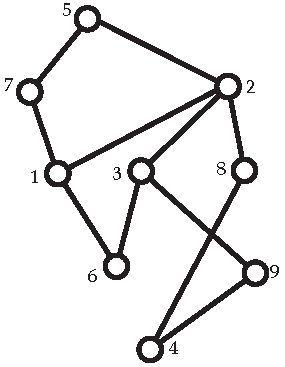
\includegraphics{posets-figs/intord_find_rep_ex4}
  \end{center}
  \caption{Is this poset an interval order?}\label{fig:intord_find_rep_ex4}
  \end{figure}
\item Find an interval representation for the poset in
  \autoref{fig:intord_find_rep_ex2} or give a reason why one does not
  exist.
  \begin{figure}[h]
  \begin{center}
    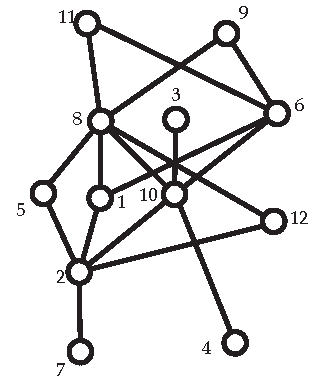
\includegraphics{posets-figs/intord_find_rep_ex2}
  \end{center}
  \caption{Is this poset an interval order?}\label{fig:intord_find_rep_ex2}
  \end{figure}
\item Find an interval representation for the poset in
  \autoref{fig:intord_find_rep_ex3} or give a reason why one does not
  exist.
  \begin{figure}[h]
  \begin{center}
    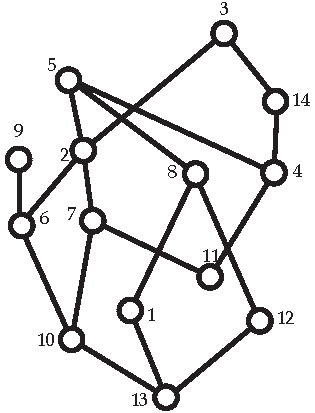
\includegraphics{posets-figs/intord_find_rep_ex3}
  \end{center}
  \caption{Is this poset an interval order?}\label{fig:intord_find_rep_ex3}
  \end{figure}
\item Use the First Fit algorithm (ordering by left endpoints) to find
  the width $w$ of the interval order shown in
  \autoref{fig:intord_firstfit_ex1} and a partition into $w$
  chains. Also give an antichain with $w$ points.
  \begin{figure}[h]
    \centering
    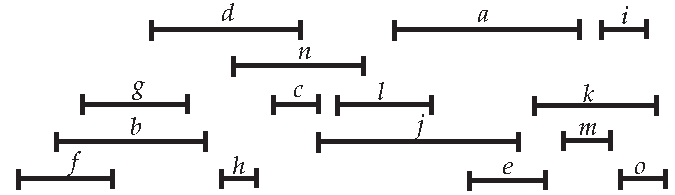
\includegraphics{posets-figs/intord_firstfit_ex1}
    \caption{An interval representation}
    \label{fig:intord_firstfit_ex1}
  \end{figure}
\end{enumerate}

%%% Local Variables: 
%%% mode: latex
%%% TeX-master: "book"
%%% End: 
